\subsection{Screw Joint}
\emph{Author: Mauro Manetti and Marco Morandini}

The screw joint is a combination of:
\begin{itemize}
\item an in line joint, that constrains one point to move along 
a line attached to another point:
\begin{align*}
	\T{e}_{1hx}^T\plbr{\T{x}_2 + \T{f}_2 - \T{x}_1 - \T{f}_1} &= 0 \\
	\T{e}_{1hy}^T\plbr{\T{x}_2 + \T{f}_2 - \T{x}_1 - \T{f}_1} &= 0
\end{align*}
where $\T{e}_{1hi}$ is the $i$-th column of matrix
$\T{R}_1 \tilde{\T{R}}_{1h}$
\begin{equation}
	\T{e}_{jhi} = \plbr{\T{R}_j \tilde{\T{R}}_{jh}}\sqbr{i}
\end{equation}
$\T{x}_j$ is the position of node $j$
and $\T{f}_j$ is the offset of the joint with respect node $j$,
both in the absolute coordinate system; the offset is constant
with respect to the reference frame of the joint,
so $\T{f}_j=\T{R}_j\tilde{\T{f}}_j$.

\item a revolute rotation joint, that constrains the relative
orientation of two nodes to be a rotation about an axis that
is fixed with respect to the two bodies:
\begin{align*}
	\T{e}_{2hx}^T \T{e}_{1hz} = 0 \\
	\T{e}_{2hy}^T \T{e}_{1hz} = 0
\end{align*}

\item a linear relationship between the relative rotation
about the common axis and the relative position along the common axis:
\begin{equation}
	\label{eq:SCREW-constraint}
	\frac{p}{2 \pi} (\theta - \theta_0 ) - \T{e}_{1hz}^T\plbr{\T{d} - \T{d}_0} = 0
\end{equation}
where the nodes distance vectors $\T{d}$ and $\T{d}_0$ can be written
as:
\begin{eqnarray}
        \nonumber 
        \T{d} &=& \T{x}_2 + \T{f}_2 - \T{x}_1 - \T{f}_1 \\
        \nonumber
        \T{d}_0 &=& \T{x}_{2_0} + \T{f}_{2_0} - \T{x}_{1_0} - \T{f}_{1_0}
\end{eqnarray}  
while $p$ represents the distance between the nodes 
along axis $\T{e}_{1hz}$ corresponding to one revolution 
about the same axis.
\end{itemize}

The rotation $\theta$ is formulated as
\begin{align}
        \label{theta_angle_definition}
	\nonumber
	\theta =& \tilde{\T{R}}_{1h3}^T \llk{ax}\plbr{\llk{exp}^{-1}\plbr{\T{R}_1^T \T{R}_2}} \\
                 \nonumber
	       =& \tilde{\T{R}}_{1h3}^T \TT{R}_1^T\llk{ax}\plbr{\llk{exp}^{-1}\plbr{\T{R}_2 \T{R}_1^T}} \\
               =& \T{e}_{1hz}^T\llk{ax}\plbr{\llk{exp}^{-1}\plbr{\T{R}_2 \T{R}_1^T}}
\end{align}
where $\tilde{\T{R}}_{1h3}$ is the third axis of the constant 
relative orientation of node 1, while $\T{e}_{1hz}$ is the screw joint axis. 
To overcome the limitation $\shbr{\theta}<\pi$, an appropriate
unwrap angle function has been implemented in the code, so allowing to
compute the right residual of Equation~(\ref{eq:SCREW-constraint}).  

The virtual perturbation of Equation~(\ref{theta_angle_definition})
can be expressed as
\begin{equation}
	\delta\theta = \tilde{\T{R}}^T_{1h3}\TT{\Gamma}\plbr{\T{\theta}}^{-1}\TT{R}^T_1\plbr{\T{\theta}_{2\delta} - \T{\theta}_{1\delta}}
\end{equation}
so the virtual perturbation of Equation~(\ref{eq:SCREW-constraint})
\begin{align}
        \nonumber
        \frac{p}{2\pi}\T{e}^T_{1hz}\TT{\Gamma}\plbr{\T{\theta}}^{-1}\TT{R}^T_1 \plbr{\T{\theta}_{2\delta} - \T{\theta}_{1\delta}}
        - \T{e}^T_{1hz}\T{d} \times \T{\theta}_{1\delta} &\\
        - \T{e}^T_{1hz} \plbr{\delta\T{x}_2 - \T{f}_2 \times \T{\theta}_{2\delta} - \delta\T{x}_1 + \T{f}_1\times \T{\theta}_{1\delta}} = 0 
        \label{eq:virtual_perturbation_const_eq}
\end{align}
yields the contribution of the constraint to the forces and moments
acting on the constrained nodes:
\begin{align}
         \T{F}_1 &= \T{e}_{1hz} \lambda \\ 
	 \T{C}_1 &= \plbr{ - \frac{p}{2\pi}\TT{R}_1\TT{\Gamma}\plbr{\T{\theta}}^{-T}\tilde{\T{R}}_{1h3} +
                           \T{f}_1 \times \T{e}_{1hz} } \lambda 
	 \label{eq:screw_couple_1}	  
	 \\
         \T{F}_2 &= -\T{e}_{1hz} \lambda \\
	 \T{C}_2 &= \plbr{ \frac{p}{2\pi}\TT{R}_1\TT{\Gamma}\plbr{\T{\theta}}^{-T}\tilde{\T{R}}_{1h3} - \T{f}_2 \times \T{e}_{1hz} } \lambda 
	 \label{eq:screw_couple_2}	  
\end{align}
where $\lambda$ is the Lagrange multiplier that here assumes the meaning
of reaction force along the screw axis.

The problem linearization requires the already computed virtual perturbation of the 
constraint equation (see Equation~(\ref{eq:virtual_perturbation_const_eq})) and 
the constraint forces and couples virtual perturbation:

\begin{align}
        \delta\T{F}_1 =& -\lambda\T{e}_{1hz} \times \T{\theta}_{1\delta} + \T{e}_{1hz} \delta\lambda  
	\label{eq:F1_virtual_variation}
	\\
        \nonumber
	\delta\T{C}_1 =& \lambda \biggl[\frac{p}{2\pi}\plbr{\TT{R}_1\TT{\Gamma}\plbr{\T{\theta}}^{-T}\tilde{\T{R}}_{1h3}}\times\T{\theta}_{1\delta} - \\ 
					\nonumber
                                        & \frac{p}{2\pi} \TT{R}_1\T{\Gamma}\plbr{\T{\theta}}^{-T}
					\TT{L}\plbr{-\T{\theta}, \TT{\Gamma}\plbr{\T{\theta}}^{-T}\tilde{\T{R}}_{1h3}}\TT{\Gamma}\plbr{\T{\theta}}^{-1}\TT{R}_1^T\plbr{\T{\theta}_{2\delta} - \T{\theta}_{1\delta}} + \\
					\nonumber
                                        & \T{e}_{1hz}\times\T{f}_1\times\T{\theta}_{1\delta} -\T{f}_1\times\T{e}_{1hz}\times\T{\theta}_{1\delta} \biggr] + \\
                                        & \frac{\T{C}_1}{\lambda} \delta\lambda\\
        \delta\T{F}_2 =& \lambda\T{e}_{1hz} \times \T{\theta}_{1\delta} - \T{e}_{1hz} \delta\lambda
	\label{eq:F2_virtual_variation}
	\\ 
        \nonumber
	\delta\T{C}_2 =& \lambda \biggl[-\frac{p}{2\pi}\plbr{\TT{R}_1\TT{\Gamma}\plbr{\T{\theta}}^{-T}\tilde{\T{R}}_{1h3}}\times\T{\theta}_{1\delta} + \\
	                           \nonumber
				   &\frac{p}{2\pi} \TT{R}_1\T{\Gamma}\plbr{\T{\theta}}^{-T} \TT{L}\plbr{-\T{\theta}, \TT{\Gamma}\plbr{\T{\theta}}^{-T}\tilde{\T{R}}_{1h3}}
				    \TT{\Gamma}\plbr{\T{\theta}}^{-1}\TT{R}_1^T\plbr{\T{\theta}_{2\delta} - \T{\theta}_{1\delta}} - \\
				    \nonumber
                                   &\T{e}_{1hz}\times\T{f}_2\times\T{\theta}_{2\delta} + \T{f}_2\times\T{e}_{1hz}\times\T{\theta}_{1\delta}    
		           \biggr] + \\
		          &\frac{\T{C}_2}{\lambda}\delta\lambda
\end{align}      
where the operator $\T{L}()$ has been introduced according to the following 
definition
\begin{equation}
  \delta\T{\Gamma}(\T{\theta})^T\T{a}= -\T{L}(-\T{\theta}, \T{a})\delta\T{\theta} 
  \label{L_definition}
\end{equation}
which can be manipulated to obtain the needed relation
\begin{align}
  \nonumber
  \delta(\TT{\Gamma}(\T{\theta})^T \TT{\Gamma}(\T{\theta})^{-T}\T{a})=&
  \delta\TT{\Gamma}(\T{\theta})^T\TT{\Gamma}(\T{\theta})^{-T}\T{a}+ \\
  \nonumber
  &\TT{\Gamma}(\T{\theta})^T\delta\TT{\Gamma}(\T{\theta})^{-T}\T{a}+ \\
  &\TT{\Gamma}(\T{\theta})^T\TT{\Gamma}(\T{\theta})^{-T}\delta\T{a}=\delta\T{a} \\
  \delta\TT{\Gamma}(\T{\theta})^{-T}\T{a}=&\delta\TT{\Gamma}(\T{\theta})^{-T}
  \TT{L}\left(-\T{\theta}, \TT{\Gamma}(\T{\theta})^{-T}\T{a}\right) \delta\T{\theta}
  \label{L_definition2}
\end{align}

Now a contribution useful to obtain previous results will be reported
\begin{align}
  \nonumber
  \delta\left(\TT{R}_1\Gamma(\T{\theta})^{-1}\tilde{\T{R}}_{1h3}\right)=&
  \delta\TT{R}_1\TT{\Gamma}(\T{\theta})^{-T}\tilde{\T{R}}_{1h3}+
  \TT{R}_1\delta\TT{\Gamma}(\T{\theta})^{-T}\tilde{\T{R}}_{1h3}\\
  \nonumber
  =&-\left(\TT{R}_1\TT{\Gamma}(\T{\theta})^{-T}\tilde{\T{R}}_{1h3}\right)_\times\T{\theta}_{1\delta}+
  \TT{R}_1\TT{\Gamma}(\T{\theta})^{-T}
  \TT{L}(-\T{\theta},\TT{\Gamma}(\T{\theta})^{-T}\tilde{\T{R}}_{1h3})\delta\T{\theta}
\end{align}

\begin{figure}[h]
  \begin{center}
    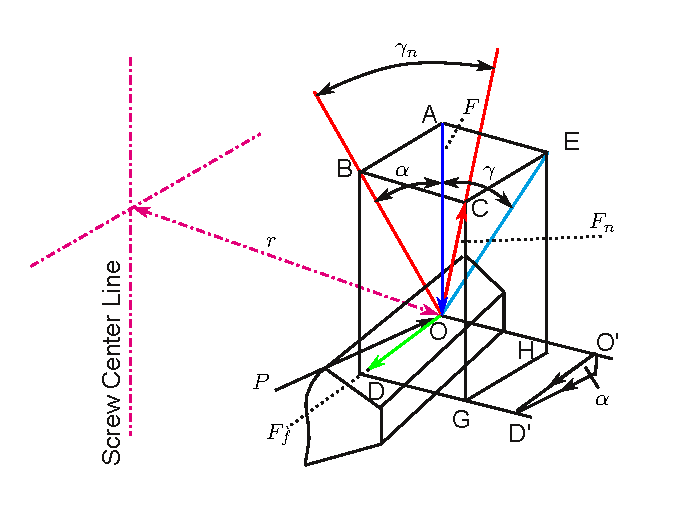
\includegraphics{Screw_sketch}
  \end{center}
  \caption{3D screw thread sketch.}
  \label{fig:screw_sketch_3D}
\end{figure}
\begin{figure}[h]
  \begin{center}
    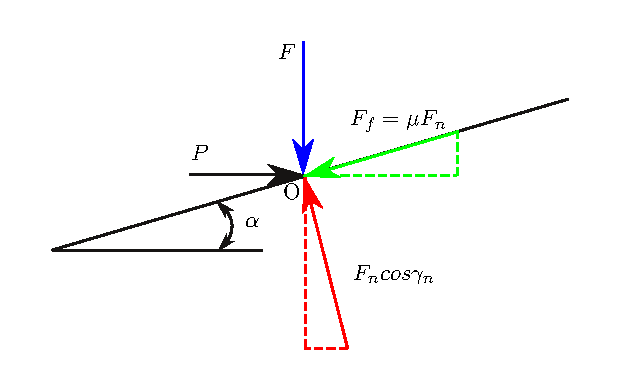
\includegraphics{Screw_sketch_2D}
  \end{center}
  \caption{2D screw thread sketch}
  \label{fig:screw_sketch_2D}
\end{figure}
This joint formulation can be improved to take into account the presence of
friction. Figures (\ref{fig:screw_sketch_3D}) and (\ref{fig:screw_sketch_2D}) show sketches 
useful to identify the forces acting on the screw thread. In the figures
the case of a screw which is raising a load $\T{F}$ is presented, the equilibrium 
equation can be written for the vertical and the horizontal directions to obtain
\begin{align}
  \T{F}+\mu\T{F}_n \sin{\alpha}=\T{F}_n \cos{\gamma_n}cos{\alpha}
  \label{eq:eq_vertical_screw}
  \\
  \T{P} = \mu\T{F}_n\cos{\alpha} + \T{F}_n\cos{\gamma_n}\sin{\alpha}
  \label{eq:eq_horizontal_screw}
\end{align}
where $\T{F}$ is the load, or the force, along the screw axis, $\T{P}$ the force acting to
rotate the screw, i.e. the torque moment over the mean thread radius $r$,
$\T{F}_n$ is the thread normal reaction, $\alpha$ the lead angle, 
and $\gamma_n$ the angle between the vectors $\T{OC}$ and $\T{OB}$ 
represented in Figure (\ref{fig:screw_sketch_3D}). 
Inside the code all the screw friction formulation is developed in function of the angle
$\gamma_n$ for convenience, anyway the usual screw informations relate the thread angle
$2\gamma$, so the joint requires as input the half thread angle $\gamma$. Looking at the Figure 
\ref{fig:screw_sketch_3D} it is possible to find the relation between these two angles
\begin{equation}
BC=AE=OA\tan{\gamma}=OB\cos{\alpha}\tan{\gamma}
\end{equation}
so
\begin{equation}
  \tan{\gamma_n}=\frac{BC}{OB}=\cos{\alpha}\tan{\gamma}
  \quad \Rightarrow \quad  
  \gamma_n=tan^{-1}(\cos{\alpha}\tan{\gamma}).
\end{equation}
From Equations 
(\ref{eq:eq_vertical_screw}) and (\ref{eq:eq_horizontal_screw}) is possible to retrive
the relation between the screw raising torque $\T{C}_r$ and the axial force $\T{F}$
\begin{equation}
  \T{C}_r=r\T{F}\left(\frac{\cos{\gamma_n}\sin{\alpha}+\mu\cos{\alpha}}
  {\cos{\gamma_n}\cos{\alpha}-\mu\sin{\alpha}}\right).
  \label{eq:raising_torque}
\end{equation}
It is easy to find the previous relation in presence of a lowering torque
\begin{equation}
  \T{C}_l=r\T{F}\left(\frac{\cos{\gamma_n}\sin{\alpha}-\mu\cos{\alpha}}
  {\cos{\gamma_n}\cos{\alpha}+\mu\sin{\alpha}}\right).
  \label{eq:lowering_torque}
\end{equation}
from which it is possible to understand the torque dependency from the
versus of the friction force $\mu\T{F}_n$. A general discriminant to apply
the right formula can be linked to the versus of the relative velocity $v$ 
between the internal and external thread and the sign of the constraint 
Lagrange multiplier $\lambda$ which represents the versus of the axial screw force
\begin{equation}
  \T{C}=r\T{F}\left(\frac{\cos{\gamma_n}\sin{\alpha}+sign(v\lambda)\,\mu\cos{\alpha}}
  {\cos{\gamma_n}\cos{\alpha}-sign(v\lambda)\,\mu\sin{\alpha}}\right).
  \label{eq:torque}
\end{equation}
Inside the code $sign(v\lambda)$ will be embedded in the friction coefficient 
computation $\mu=\mu(v, \T{F})$, so in the following for brevity it will be removed
from equations introducing the notation $\T{C}=\T{C}(\mu)$.

The torque acting on the screw for the friction presence
can now be computed as
\begin{equation}
  \T{C}_{frc}(\mu)=\T{C}(\mu)-\T{C}(0)=r\T{F}\left[\frac{\mu\sec{\gamma_n}(1+\tan^2{\alpha})}{1-\mu\sec{\gamma_n}\tan{\alpha}}\right].
  \label{eq_torque_friction}
\end{equation}
Equation (\ref{eq_torque_friction}) can be used to add
the torque friction contribution to the couples acting on the constrained
nodes reported in Equations (\ref{eq:screw_couple_1}) and (\ref{eq:screw_couple_2})
\begin{align}
  \T{C}_{1_{frc}}=\T{C}_1-\T{C}_{frc}(\mu)= \T{C}_1-r\T{F}_1\left[\frac{\mu\sec{\gamma_n}(1+\tan^2{\alpha})}{1-\mu\sec{\gamma_n}\tan{\alpha}}\right] 
  \label{eq:screw_couple_tot_1}
  \\
  \T{C}_{2_{frc}}=\T{C}_2-\T{C}_{frc}(\mu)= \T{C}_2-r\T{F}_2\left[\frac{\mu\sec{\gamma_n}(1+\tan^2{\alpha})}{1-\mu\sec{\gamma_n}\tan{\alpha}}\right] 
  \label{eq:screw_couple_tot_2}
\end{align}

At this point the only further required informations regard the relative
velocity $v$ and the virtual variation of the friction torque
contribution. Starting from the already used formula
\begin{equation}
  \delta\T{\theta}=\TT{\Gamma}(\T{\theta})^{-1}\TT{R}^T_1(\T{\theta}_{2\delta}-\T{\theta}_{1\delta})
\end{equation}
it is possible to write the following relation
\begin{equation}
  \dot{\T{\theta}}=\TT{\Gamma}(\T{\theta})^{-1}\TT{R}^T_1
                   (\TT{\Gamma}(\T{\theta}_2)\dot{\T{\theta}}_{2}-\TT{\Gamma}(\T{\theta}_1)\dot{\T{\theta}}_{1}).
\end{equation}
The angular velocity vector is defined as
\begin{equation}
  \T{\omega}_{\theta}=\TT{\Gamma}(\T{\theta})\dot{\T{\theta}}=\TT{\Gamma}(\T{\theta})\TT{\Gamma}(\T{\theta})^{-1}\TT{R}^T_1
                      (\TT{\Gamma}(\T{\theta}_2)\dot{\T{\theta}}_{2}-\TT{\Gamma}(\T{\theta}_1)\dot{\T{\theta}}_{1})
                     = \TT{R}^T_1(\T{\omega}_{2}-\T{\omega}_{1})
\end{equation}
from which the angular velocity modulus with sign can be obtained
\begin{equation}
  \omega_{\theta}=\tilde{\T{R}}_{1h3}^T\T{\omega}_{\theta}=\tilde{\T{R}}_{1h3}^T\TT{R}_1^T(\T{\omega_2}-\T{\omega}_1).
\end{equation}
Now the relative velocity on the screw thread, along the friction force direction, can be 
written as
\begin{equation}
  v=\omega_\theta r\cos{\alpha}=\tilde{\T{R}}_{1h3}^T\TT{R}_1^T(\T{\omega_2}-\T{\omega}_1)r\cos{\alpha}.
\end{equation} 
The virtual perturbation of the friction couple is required to write the 
linearized problem
\begin{align}
  \nonumber
  \delta\T{C}_{frc}=&\delta\T{F}r\left[\frac{\mu\sec{\gamma_n}(1+\tan^2{\alpha})}{1-\mu\sec{\gamma_n}\tan{\alpha}}\right]+\\
                    \nonumber
                    &\T{F}r\left[\frac{\sec{\gamma_n}(1+\tan^2{\alpha})}{1-\mu\sec{\gamma_n}\tan{\alpha}}+
		    \frac{\mu\sec{\gamma_n}(1+\tan^2{\alpha})}{\left(1-\mu\sec{\gamma_n}\tan{\alpha}\right)^2}
		    \sec{\gamma_n}\tan{\alpha}\right]
		    \delta\mu\\
		    =&r\left[\frac{\mu\sec{\gamma_n}(1+\tan^2{\alpha})}{1-\mu\sec{\gamma_n}\tan{\alpha}}\right]\delta\T{F}+
		     \T{F}r\left[\frac{\mu\sec{\gamma_n}(1+\tan^2{\alpha})}{\left(1-\mu\sec{\gamma_n}\tan{\alpha}\right)^2}\right]
		     \delta\mu
\end{align}
where the friction coefficient virtual variation is automatically computed by the code,
once provided the $F$ and $\mu$ virtual perturbations
\begin{equation}
  \delta\mu=\delta\mu(\delta\T{F}, \delta v).
\end{equation}
Anyway the screw axial forces virtual variations have already been reported in Equations
\ref{eq:F1_virtual_variation} and \ref{eq:F2_virtual_variation}, so to complete the problem description is just required the 
definition of the relative velocity virtual perturbation 
\begin{align}
  \nonumber
  \delta v=&\tilde{\T{R}}_{1h3}^T\delta\TT{R}_1^T(\T{\omega}_2-\T{\omega}_1)r\cos{\alpha}+
            \tilde{\T{R}}_{1h3}^T\TT{R}_1^T(\delta\T{\omega}_2-\delta\T{\omega}_1)r\cos{\alpha} \\
	  =& r\cos{\alpha}\tilde{\T{R}}_{1h3}^T
	      \TT{R}_1^T\left(\T{\omega}_2-\T{\omega}_1\right)_{\times}\T{\theta}_{1\delta}+
	      r\cos{\alpha}\tilde{\T{R}}_{1h3}^T\left(\delta\T{\omega}_2-\delta\T{\omega}_1\right).
\end{align}



\paragraph{Physics.}
In other words, node 1 is the screw and node 2 is the bolt;
neglecting the offset, the force along the screw axis is related
to the couple about the same axis by the relationship
\begin{equation}
	C = - \frac{p}{2\pi} F
\end{equation}
which results from a power balance
\begin{equation}
  C \omega_\theta + F v_{lin} = 0
\end{equation}
in terms of relative linear ($v_{lin}$) and angular ($\omega_\theta$) velocity,
with the kinematic relationship
\begin{equation} 
  v_{lin} = \frac{p}{2\pi} \omega_\theta
\end{equation}

